\section{The Lifecycle of Software Update}
A \emph{software update (SU)} is the unit of change for the blockchain software. It must have a clear goal of what it tries to achieve and why it would be beneficial, if applied to the system. Moreover, it should have a clear scope. In Figure \ref{lifecycle}, we depict the full lifecycle of a software update following a decentralized approach.
In this lifecycle, we identify four distinct phases: a) the \emph{ideation phase}, b) the \emph{implementation phase}, c) the \emph{approval phase} and d) the \emph{activation phase}. In this section, we briefly outline each phase and at the subsequent sections we provide all necessary details for realizing each phase in a decentralized setting.

Interestingly, the phases in the lifecycle of a SU are essentially independent from the approach (centralized or decentralized) that we follow. They constitute intuitive steps in a software lifecycle process that starts from the initial idea conception and ends at the actual activation of the change on the client software. Based on this observation, one can examine each phase and compare the traditional centralized approach, used to implement it, to its decentralized alternative. Moreover, not all phases need to be decentralized in a real world scenario. One has to measure the trade-off between decentralization benefits versus practicality and decide what phases will be decentralized. Our decomposition of the lifecycle of a SU in distinct phases helps towards this direction.

\begin{figure}[H]
    \caption{The lifecycle of a software update (a decentralized approach)}
    \centering
    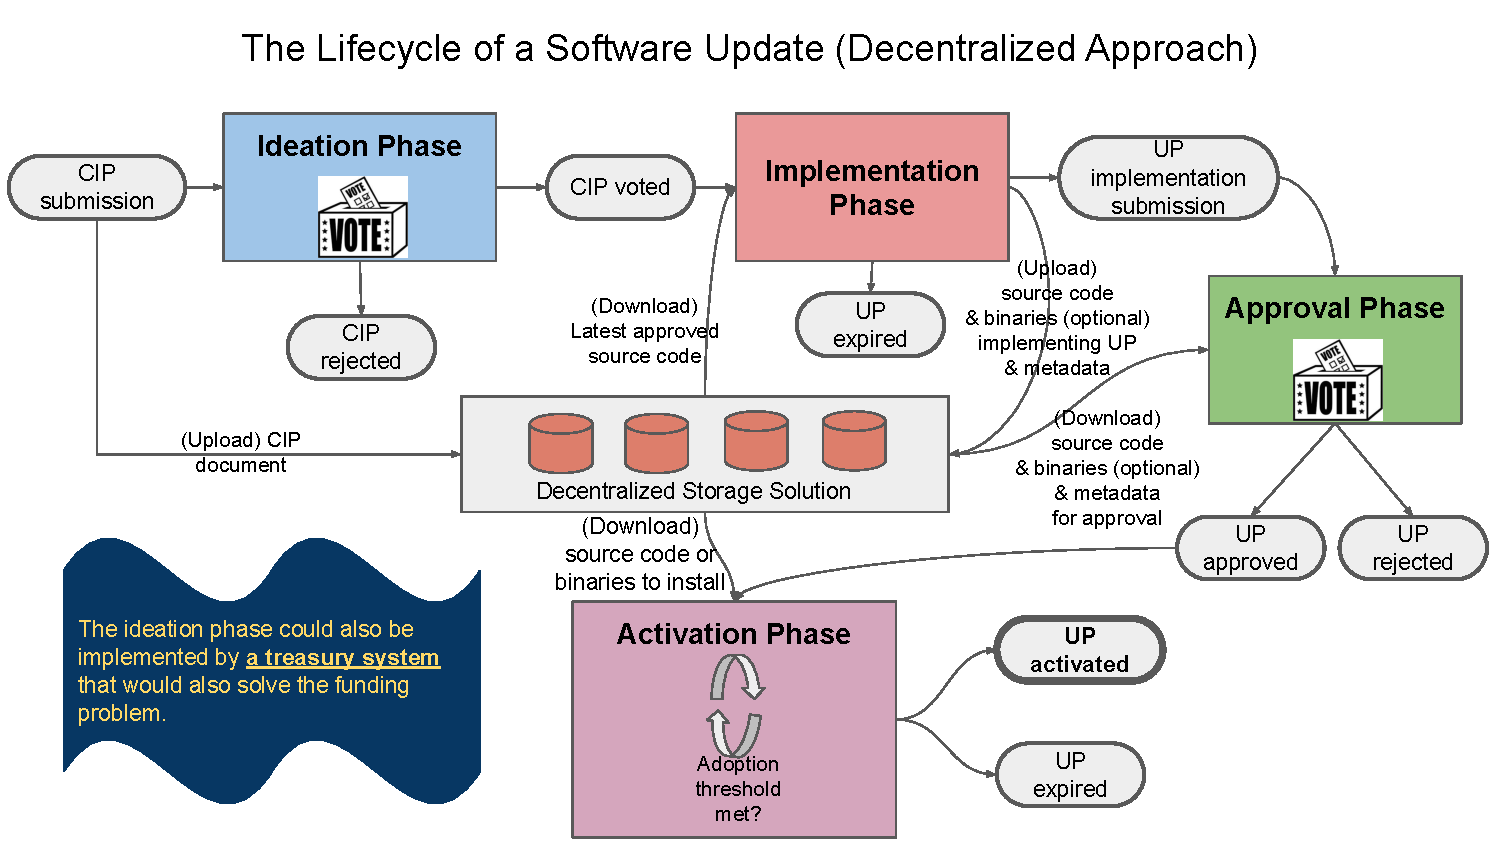
\includegraphics[width=0.9 \columnwidth,keepaspectratio]{figures/lifecycle_phases.pdf}
    \label{lifecycle}
\end{figure}

\subsection{Ideation}
%\paragraph{Scope of the phase.} 
A SU starts as an idea. Someone captures the idea of implementing a change that will serve a specific purpose (fix a bug, implement a new feature, provide some change in the consensus protocol, perform some optimization etc.). 
The primary goal of this phase is to capture the idea behind a SU, then record the justification and scope of the SU in some appropriate documentation and finally come to a decision on the priority that will be given to this SU. 
%In Figure \ref{lifecycle}, we call this documentation a \emph{SIP (Software  \footnote{''Software'' and ''System'' are two terms that could be considered equivalent for the scope of this paper and we intend to use them interchangeably. For example, a SIP could also stand for a System Improvement Proposal} Improvement Document)}.

%\paragraph{Centralized approach.}
Traditionally, in the centralized approach, a SU is proposed by some central authority (original author, group of authors, package maintainer etc.), who essentially records the need for a specific SU and then decides when (or, in which version) this could be released. In many cases, (e.g., Bitcoin \cite{bitcoin}, Ethereum \cite{ethereum}) the relevant SU justification document (called BIP, or EIP respectively) is submitted to the community, in order to be discussed. Even when this ''social alignment'' step is included in this phase, the ultimate decision (which might take place at a later phase in the lifecycle), for the proposed SU, is taken by the central authority. Therefore, the road-map for the system evolution is effectively decided centrally. Moreover, this social consensus approach is informal (i.e., not part of a protocol, or output of an algorithm) and is not recorded on-chain as an immutable historical event.

%\paragraph{Decentralized approach.}
The ideation phase in the decentralized approach is depicted in Figure \ref{ideation}.

\begin{figure}[H]
    \caption{The ideation phase.}
    \centering
    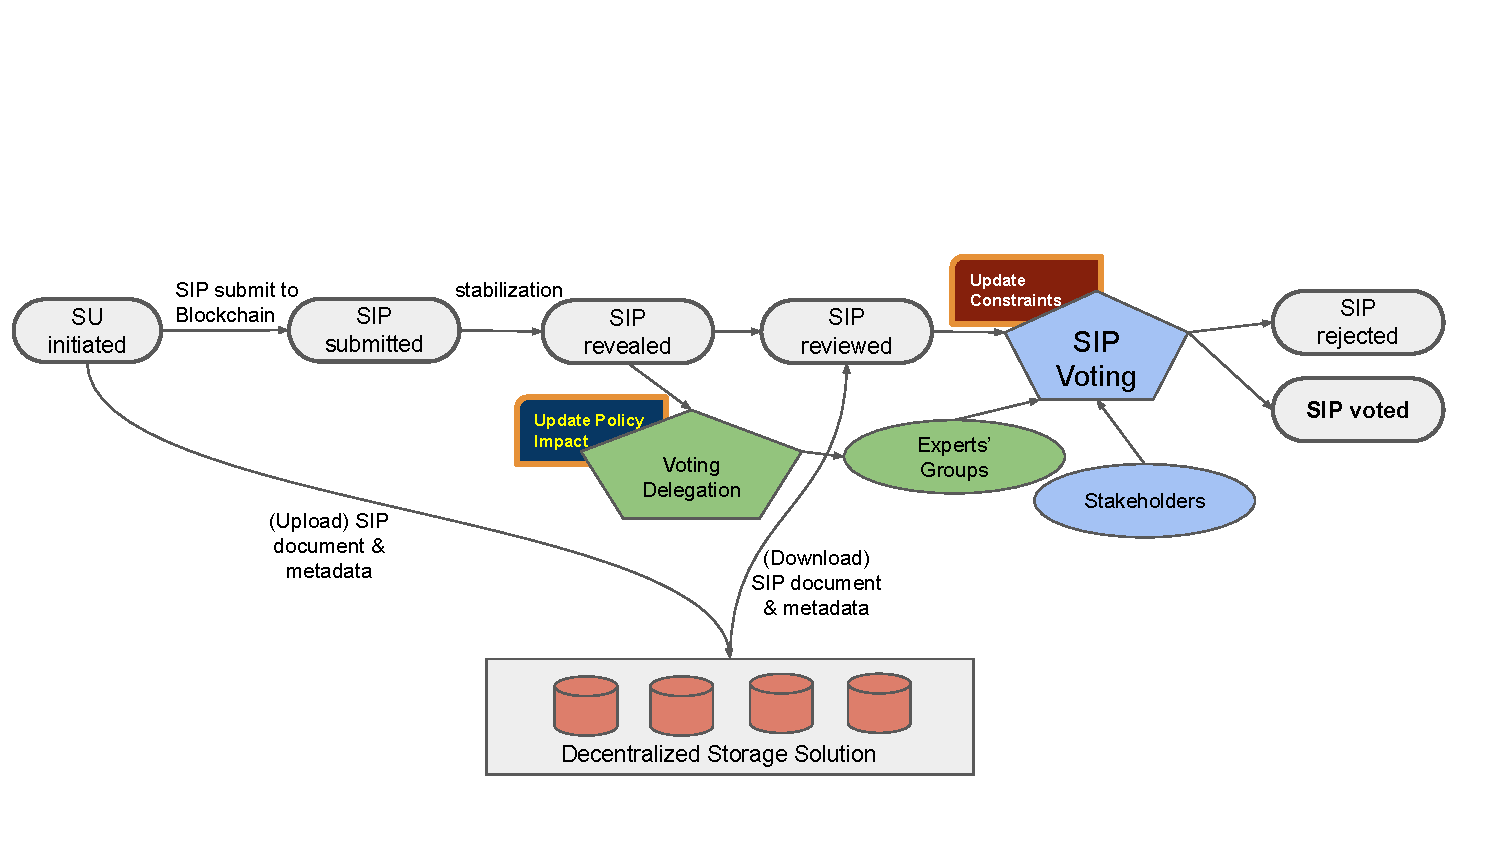
\includegraphics[width=0.9 \columnwidth,keepaspectratio]{figures/ideation_phase.pdf}
    \label{ideation}
\end{figure}

In the decentralized setting a SU starts its life as an idea for improvement of the blockchain system, which is recorded in a human readable simple text document, called the \emph{SIP (Software  \footnote{''Software'' and ''System'' are two terms that could be considered equivalent for the scope of this paper and we intend to use them interchangeably. For example, a SIP could also stand for a System Improvement Proposal} Improvement Document)}. The SU life starts by submitting the corresponding SIP to the blockchain by means of a special fee-supported transaction. Any stakeholder can potentially submit a SIP and thus propose a SU. 
%\emph{CIP}, which stands for \emph{Cardano Improvement Proposal}\footnote{We have used the Cardano \citep{cardano} blockchain system as an example of a stake-based ledger.}. 

A SIP includes basic information about a SU, such as the title, a description, the author(s) etc. Its sole purpose is to justify the necessity of the proposed software update and try to raise awareness and support from the community of users. A SIP must also include all necessary information that will enable the SU validation against previous SUs (e.g., update dependencies or update conflict issues), or against any prerequisites required, in order to be applied.

A SIP is initially uploaded to some external (to the blockchain system) decentralized storage solution\footnote{We will come back to this in the corresponding section} and a hash id is generated, in order to uniquely identify it. This hash id is committed to the blockchain in a two-step approach following a hash-based commitment scheme, in order to preserve the rightful authorship of the SIP.

Once the SIP is revealed a voting period for the specific proposal is initiated. Any stakeholder is eligible to vote for a SIP and the voting power will be proportional to his/her stake. Votes are specialized fee-supported transactions, which are committed to the blockchain.

Note that since a SIP is a document justifying the purpose and benefit of the proposed software update, it should not require in general sufficient technical expertise, in order for a stakeholder to review it and decide on his/her vote. However, in the case that the evaluation of a SIP requires greater technical knowledge, then a voting delegation mechanism exists. This means that a stakeholder can delegate his/her voting rights to an appropriate group of experts but also preserving the right to override the delegate's vote, if he/she wishes. 

The delegation mechanism will also be used in order to implement the concept of an \emph{update policy} that will be described in a later section and enables different activation speeds for a SU depending on its type (e.g., a bug-fix versus a change request, a SU that has a consensus protocol impact versus a no-impact one, etc.). For all these special \emph{delegation groups} will be considered, as we will discuss in the relevant section. A SIP after the voting period can either be voted or rejected. Details on the voting and delegation protocols can be found in the relevant section.

Note that in the decentralized approach the ideation phase could very well be implemented by a treasury system (e.g., similar to the one proposed by Bingsheng et al. \cite{cryptoeprint:2018:435}). This would enable additionally the appropriate management of the funding of each SU.

\subsection{Implementation}
%\nnote{When source code is submitted for approval this is conceptually equivalent to a Github pull request}
%
%\nnote{The source code in order to be voted must include all previous approved UPs up to the moment of UP submission. This is conceptually equivalent to a merge of a Pull Request (i.e., of a branch implementing the UP) to the master (i.e., main) base branch, which accumulates all approved UPs. Although, in our case there is no single master branch, instead there are multiple different ''versions'' of master branches and the community must reach at a consensus, which one will prevail.}

The voting of a SIP is the green light signal for entering the implementation phase. This is the period where the actual implementation of a SIP takes place. So one could very roughly imagine this phase as a box, where a SIP comes in as input and source code implementing the SIP comes out as output.

%\paragraph{Scope of this phase.}
The scope of this phase is twofold: a) to develop the source code changes that implement a specific voted SIP and b) to execute a second voting delegation round, in order to identify the experts that will approve the new source code. At the end of this phase, the developer creates a bundle comprising the new source code and the accompanied metadata, which we call an \emph{update proposal (UP)}. The newly created UP must be submitted for approval, in order to move forward.

%\paragraph{Centralized approach.}
In the centralized setting, it is typical (in the context of an open source software development model), when a developer wants to implement a change, first to download from a central code repository the version of the source code that will be the base for the implementation and then, when the implementation is finished, to upload it to the same central code repository and submit a pull-request. The latter is essentially a call for approval for the submitted code. The central authority responsible for the maintenance of the code-base, must review the submitted code and decide, if it will be accepted, or not. Therefore, in the centralized approach the implementation phase ends with the submission of a pull-request.

%\paragraph{Decentralized approach}
The decentralized alternative for the implementation phase is identical to its centralized counterpart as far as the development of the new code is concerned. However, in the decentralized setting, there exist these major differences:
a) there is not a centrally-owned code repository (since there is not a central authority responsible for the maintenance of the code), b) a delegation process is executed, in parallel to the implementation, as a preparation step for the (decentralized) approval phase that will follow and c) the conceptual equivalent to the submission of a pull-request must be realized.

\begin{figure}[H]
    \caption{The implementation phase.}
    \centering
    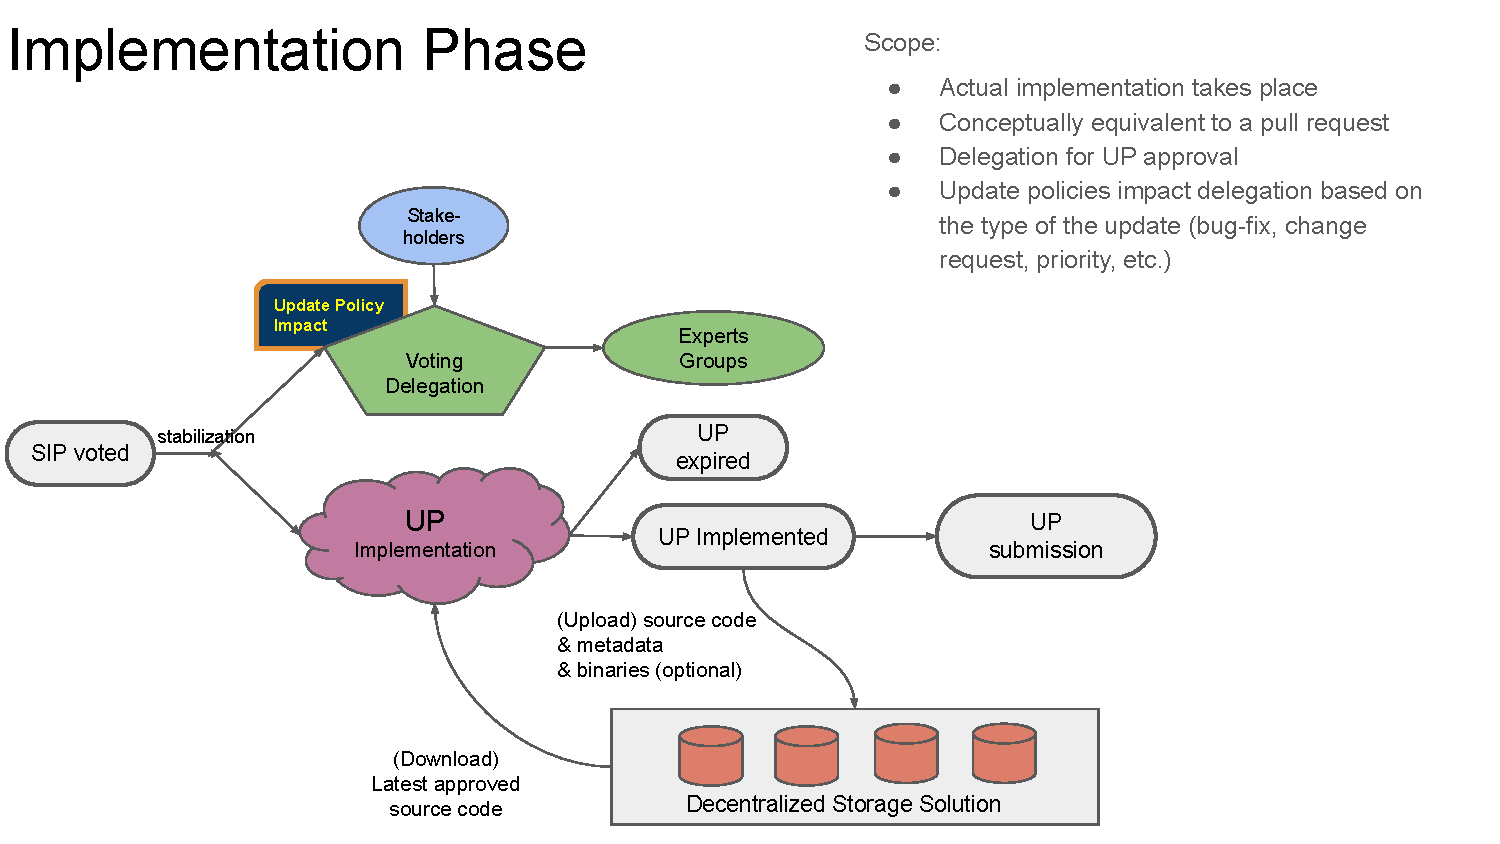
\includegraphics[width=0.9 \columnwidth,keepaspectratio]{figures/implementation_phase.pdf}
    \label{implementation}
\end{figure}

In Figure \ref{implementation} we depict the decentralized implementation phase. Similar to the centralized case, the implementation of a change must be based on some existing code, which we call the base source code, which the developer must download locally, in order to initiate the implementation. However, in the decentralized setting there is not a centrally-owned code repository. All the approved versions of the code are committed into the blockchain. Therefore, we assume that the developer finds the appropriate (usually the latest) approved base source code in the blockchain and downloads it locally, using the link to the developer-owned code repository provided in the UP metadata. We abstract this code repository in Figure \ref{implementation} with the depicted decentralized storage solution.

It is true that the review of source code is a task that requires extensive technical skills and experience. Therefore, it is not a task that can be assumed by the broad base of the stakeholders community. A voting delegation mechanism at this point must be in place, to enable the delegation of the strenuous code-approval task to some group of experts. In a similar logic with the delegation process, within the ideation phase, discussed above, the delegation process could be leveraged to implement different update policies per type of software update.

As we have seen, the voting approval of a SIP signals the beginning of the implementation phase for this SIP. The SIP has an estimated implementation elapsed time that was included in the SIP metadata, submitted along with the SIP at the ideation phase. This time period, increased by a contingency parameter, will be the available time window for a SIP to be implemented. Upon the conclusion of the implementation, a bundled (source code and metadata) UP is created. The UP must be uploaded to some (developer-owned) code repository and a content-based hash id must be produced that will uniquely identify the UP. This hash id will be submitted to the blockchain as a signal for a request to approval. This is accomplished with a specialized fee-supported  transaction, which represents the decentralized equivalent to a pull-request. SIPs that fail to be implemented within the required time framework, will result to expired UPs and the SIP must be resubmitted to the ideation phase, as a new proposal. The UP submission transaction signals the entering into the approval phase.


\subsection{Approval}

\nnote{The voter at this phase votes for three things: a) for the correspondence of the source code to the CIP (i.e., authenticity testing / security auditing), b) For the inclusion from the new source code of all previous approved UPs (i.e., regression testing), c) The correctness of the new code (i.e., testing)}

\nnote{If there is also a binary upload for a specific platform for a UP, then the approval must vote for the authenticity and safety of the binaries as well. This might require a re-delegation to a specialized team for the specific platform. So this could be a separate vote}

\subsection{Activation}




